% !TeX root = er.tex

\chapter{Navegação com base em mapeamento}\label{ch.map-based}

Agora que temos um mapa, seja fornecido pelo usuário ou descoberto pelo robô, podemos discutir \emph{planejamento do caminho}, um algoritmo de nível superior. Considere um robô usado em um hospital para o transporte de medicamentos e outros suprimentos das áreas de armazenamento para os médicos e enfermeiros. Dada uma destas tarefas, qual é a melhor maneira de ir do ponto A para o ponto B. Pode haver várias maneiras de se mover pelos corredores para chegar ao objetivo, mas também pode haver caminhos curtos que o robô não está autorizado a tomar, por exemplo, caminhos que passam por corredores próximos às salas de cirurgia.

Apresentamos três algoritmos para planejar o caminho mais curto desde uma posição inicial até uma posição de objetivo, assumindo que temos um mapa da área que indica as posições dos obstáculos na área. Edsgar W. Dijkstra, um dos pioneiros da ciência da computação, propôs um algoritmo para o problema do caminho mais curto. A seção~\ref{s.dijkstra-grid} descreve o algoritmo para um mapa de grade, enquanto a seção~\ref{s.dijkstra-continuous} descreve o algoritmo para um mapa contínuo. O algoritmo \astar{}, um aperfeiçoamento do algoritmo de Dijkstra baseado em métodos heurísticos, é apresentado na seção~\ref{s.astar}. Finalmente, a seção~\ref{s.path-and-obstacle} discute como combinar um algoritmo de alto nível de planejamento de caminhos com um algoritmo de baixo nível para evitar obstáculos.

\section{Algoritmo de Dijkstra para um mapa de grade}\label{s.dijkstra-grid}

Dijkstra descreveu seu algoritmo para um gráfico discreto de nós e bordas. Aqui nós o descrevemos para um mapa de células em grade (Fig.~ ~ref{fig.dijkstra-grid}). A célula {S} é a célula inicial do robô e sua tarefa é mover-se para a célula de objetivo \p{G}. As células que contêm obstáculos são mostradas em preto. O robô pode sentir e mover-se para um \emph{vizinho} da célula \p{c} que ele ocupa. Para simplificar, especificamos que os vizinhos da cela são as quatro células próximas a ela horizontal e verticalmente, mas não diagonalmente. A figura~\ref{fig.dijkstra-path} mostra um trajeto mais curto de {S] para {G}:
\[
\begin{array}{ll}
(4,0) \rightarrow &(4,1)\rightarrow (3,1) \rightarrow (2,1) \rightarrow (2,2) \rightarrow \\
&(2,3) \rightarrow (3,3) \rightarrow (3,4) \rightarrow (3,5) \rightarrow (4,5)\,.
\end{array}
\]

\begin{figure}
\begin{minipage}{.5\textwidth}
\begin{tikzpicture}[scale=.8]
\pic[scale=.8,draw] at (0,0) {astar};
\end{tikzpicture}
\caption{Mapa de grade para o algoritmo da Dijkstra}
\label{fig.dijkstra-grid}
\end{minipage}
\hspace{\fill}
\begin{minipage}{.5\textwidth}
\begin{tikzpicture}[scale=.8]
\pic[scale=.8,draw] at (0,0) {astar};
\begin{scope}[xshift=.5cm,yshift=.5cm]
\draw[->,thick,blue] (.2,0) -- (1,0);
\draw[->,thick,blue] (1,0) -- (1,1);
\draw[->,thick,blue] (1,1) -- (1,2);
\draw[->,thick,blue] (1,2) -- (2,2);
\draw[->,thick,blue] (2,2) -- (3,2);
\draw[->,thick,blue] (3,2) -- (3,1);
\draw[->,thick,blue] (3,1) -- (4,1);
\draw[->,thick,blue] (4,1) -- (5,1);
\draw[->,thick,blue] (5,1) -- (5,.2);
\end{scope}
\end{tikzpicture}
\caption{O caminho mais curto encontrado pelo algoritmo da Dijkstra}
\label{fig.dijkstra-path}
\end{minipage}
\end{figure}

%\begin{figure}
%\subfigures
%\begin{minipage}{\textwidth}
%\leftfigure[c]{
%\begin{tikzpicture}[scale=.8]
%\pic[scale=.8] at (0,0) {astar};
%\end{tikzpicture}
%}
%\hspace{\fill}
%\rightfigure[c]{
%\begin{tikzpicture}[scale=.8]
%\pic[scale=.8] at (0,0) {astar};
%\begin{scope}[xshift=.5cm,yshift=.5cm]
%\draw[->,thick,blue] (.2,0) -- (1,0);
%\draw[->,thick,blue] (1,0) -- (1,1);
%\draw[->,thick,blue] (1,1) -- (1,2);
%\draw[->,thick,blue] (1,2) -- (2,2);
%\draw[->,thick,blue] (2,2) -- (3,2);
%\draw[->,thick,blue] (3,2) -- (3,1);
%\draw[->,thick,blue] (3,1) -- (4,1);
%\draw[->,thick,blue] (4,1) -- (5,1);
%\draw[->,thick,blue] (5,1) -- (5,.2);
%\end{scope}
%\end{tikzpicture}
%}
%\leftcaption{Grid map for Dijkstra's algorithm}\label{fig.dijkstra-grid}\rightcaption{The shortest path found by Dijkstra's algorithm}\label{fig.dijkstra-path}
%\end{minipage}
%\end{figure}

Duas versões do algoritmo são apresentadas: A primeira é para redes em que o custo da mudança de uma célula para uma de suas vizinhas é constante. Na segunda versão, cada célula pode ter um custo diferente associado à mudança para ela, portanto o caminho mais curto geometricamente não é necessariamente o caminho mais curto quando os custos são levados em conta.

\subsection{O algoritmo de Dijkstra em um mapa de grade com custo constante}

Algoritmo~\ref{alg.dijkstra-grid} é o algoritmo de Dijkstra para um mapa de grade. O algoritmo é demonstrado no mapa de grade de $5 \times 6$ em Fig.~\ref{fig.dijkstra-simple}. Há três obstáculos representados pelas células negras.

\begin{figure}
\begin{alg}{O algoritmo de Dijkstra em um mapa de grade}{dijkstra-grid}
&\idv{}integer n \ass 0&// Distance from start\\
&\idv{}cell array grid \ass all unmarked&// Grid map\\
&\idv{}cell list path \ass empty&// Shortest path\\
&\idv{}cell current&// Current cell in path\\
&\idv{}cell c&// Index over cells\\
&\idv{}cell S \ass $\cdots$&// Source cell\\
&\idv{}cell G \ass $\cdots$&// Goal cell\\
\hline
\stl{}&mark S with n&\\
\stl{}&while G is unmarked&\\
\stl{}&\idc{}n \ass n $+$ 1&\\
\stl{}&\idc{}for each unmarked cell c in grid&\\
\stl{}&\idc{}\idc{}\idc{}next to a marked cell&\\
\stl{}&\idc{}\idc{}mark c with n&\\
\stl{}&current \ass G&\\
\stl{}&append current to path&\\
\stl{}&while S not in path&\\
\stl{}&\idc{}append lowest marked neighbor c&\\
\stl{}&\idc{}\idc{}of current to path&\\
\stl{}&\idc{}current \ass c&\\
\end{alg}
\end{figure}

\begin{figure}
\begin{minipage}{.5\textwidth}
\begin{tikzpicture}[scale=.8]
\pic[scale=.8,draw] at (0,0) {astar};
\end{tikzpicture}
\caption{Mapa de grade para o algoritmo da Dijkstra}
\label{fig.dijkstra-simple}
\end{minipage}
\hspace{\fill}
\begin{minipage}{.5\textwidth}
\begin{tikzpicture}[scale=.8]
\pic[scale=.8,draw] at (0,0) {astar};
\foreach \x/\y/\n in {0/0/0, 1/0/1, 0/1/1, 1/1/2, 0/2/2}
  \node at (\x+.2,\y+.8) {\p{\n}};
\end{tikzpicture}
\caption{As duas primeiras iterações do algoritmo de Dijkstra}
\label{fig.dijkstra-simple-2}
\end{minipage}
\end{figure}

%\begin{figure}
%\subfigures
%\begin{minipage}{\textwidth}
%\leftfigure[c]{
%\begin{tikzpicture}[scale=.8]
%\pic[scale=.8] at (0,0) {astar};
%\end{tikzpicture}
%}
%\hspace{\fill}
%\rightfigure[c]{
%\begin{tikzpicture}[scale=.8]
%\pic[scale=.8] at (0,0) {astar};
%\foreach \x/\y/\n in {0/0/0, 1/0/1, 0/1/1, 1/1/2, 0/2/2}
%  \node at (\x+.2,\y+.8) {\p{\n}};
%\end{tikzpicture}
%}
%\leftcaption{Grid map for Dijkstra's algorithm}\label{fig.dijkstra-simple}
%\rightcaption{The first two iterations of Dijkstra's algorithm}\label{fig.dijkstra-simple-2}
%\end{minipage}
%\end{figure}

O algoritmo marca incrementalmente cada célula \p{c} com o número de passos necessários para alcançar \p{c} a partir da célula inicial \p{S}. Nas figuras, a contagem dos passos é mostrada como um número no canto superior esquerdo de uma célula. Inicialmente, marque a célula \p{S} com $0$ já que não são necessários passos para chegar \p{S} a partir de \p{S}. Agora, marque cada vizinho de \p{S} com $1$, pois eles estão a um passo de distância de \p{S}; depois marque cada vizinho de uma célula marcada com $1$ com $2$. A figura~\ref{fig.dijkstra-simple-2} mostra o mapa da grade após estas duas iterações do algoritmo.

\begin{figure}
\begin{minipage}{.5\textwidth}
\begin{tikzpicture}[scale=.8]
\pic[scale=.8,draw] at (0,0) {astar};
\foreach \x/\y/\n in {0/0/0, 1/0/1, 0/1/1, 1/1/2, 0/2/2, 0/3/3, 1/2/3, 0/4/4, 1/3/4, 2/2/4, 3/2/5, 1/4/5}
  \node at (\x+.2,\y+.8) {\p{\n}};
\end{tikzpicture}
\caption{Após cinco iterações do algoritmo de Dijkstra}
\label{fig.dijkstra-simple-5}
\end{minipage}
\hspace{\fill}
\begin{minipage}{.5\textwidth}
\begin{tikzpicture}[scale=.8]
\foreach \x/\y in {0/0, 1/0, 1/1, 1/2, 2/2, 3/2, 3/1, 4/1, 5/1, 5/0}
  \draw[fill,lightgray] (\x,\y) rectangle +(1,1);
\pic[scale=.8,draw] at (0,0) {astar};
\foreach \x/\y/\n in {0/0/0, 1/0/1, 0/1/1, 1/1/2, 0/2/2, 0/3/3, 1/2/3, 0/4/4, 1/3/4, 2/2/4, 3/2/5, 1/4/5, 3/3/6, 3/1/6, 3/4/7, 3/0/7, 4/1/7, 4/3/7, 4/0/8, 5/3/8, 4/4/8, 5/1/8, 5/4/9, 5/0/9}
  \node at (\x+.2,\y+.8) {\p{\n}};
\end{tikzpicture}
\caption{O mapa final da grade com o caminho mais curto marcado}
\label{fig.dijkstra-simple-9}
\end{minipage}
\end{figure}

%\begin{figure}
%\subfigures
%\begin{minipage}{\textwidth}
%\leftfigure[c]{
%\begin{tikzpicture}[scale=.8]
%\pic[scale=.8] at (0,0) {astar};
%\foreach \x/\y/\n in {0/0/0, 1/0/1, 0/1/1, 1/1/2, 0/2/2, 0/3/3, 1/2/3, 0/4/4, 1/3/4, 2/2/4, 3/2/5, 1/4/5}
%  \node at (\x+.2,\y+.8) {\p{\n}};
%\end{tikzpicture}
%}
%\hspace{\fill}
%\rightfigure[c]{
%\begin{tikzpicture}[scale=.8]
%\foreach \x/\y in {0/0, 1/0, 1/1, 1/2, 2/2, 3/2, 3/1, 4/1, 5/1, 5/0}
%  \draw[fill,lightgray] (\x,\y) rectangle +(1,1);
%\pic[scale=.8] at (0,0) {astar};
%\foreach \x/\y/\n in {0/0/0, 1/0/1, 0/1/1, 1/1/2, 0/2/2, 0/3/3, 1/2/3, 0/4/4, 1/3/4, 2/2/4, 3/2/5, 1/4/5, 3/3/6, 3/1/6, 3/4/7, 3/0/7, 4/1/7, 4/3/7, 4/0/8, 5/3/8, 4/4/8, 5/1/8, 5/4/9, 5/0/9}
%  \node at (\x+.2,\y+.8) {\p{\n}};
%\end{tikzpicture}
%}
%\leftcaption{After five iterations of Dijkstra's algorithm\label{fig.dijkstra-simple-5}}
%\rightcaption{The final grid map with the shortest path marked\label{fig.dijkstra-simple-9}}
%\end{minipage}
%\end{figure}

O algoritmo continua iterativamente: se uma célula é marcada com $n$, seus vizinhos não marcados são marcados com $n+1$. Quando o \p{G} está finalmente marcado, sabemos que a distância mais curta entre \p{S} e \p{G} é $n$. Fig.~\ref{fig.dijkstra-simple-5} mostra o mapa da grade após cinco iterações e Fig.~\ref{fig.dijkstra-simple-9} mostra o mapa da grade final após nove iterações quando a célula de objetivo foi atingida.

Agora é fácil encontrar um caminho mais curto trabalhando para trás a partir da célula de objetivo \p{G}. Na Fig.~\ref{fig.dijkstra-simple-9} um caminho mais curto consiste nas células que são coloridas de cinza. Começando com a célula de objetivo na coordenada $(4,5)$, a célula anterior deve ser ou $(4,4)$ ou $(3,5)$ já que elas estão a oito passos do início. (Isto mostra que há mais de um caminho mais curto.) Nós escolhemos arbitrariamente $(3,5)$. De cada célula selecionada marcada com $n$, escolhemos uma célula marcada com $n-1$ até que a célula \p{S} marcada com $0$ seja selecionada. A lista das células selecionadas é:
\[
(4,5),\, (3,5),\, (3,4),\, (3,3),\, (2,3),\, (2,2),\, (2,1),\, (3,1),\, (4,1),\, (4,0)\,.
\]
Invertendo a lista, obtém-se o caminho mais curto de \p{S} para \p{G}. Verifique se este é o mesmo caminho que encontramos intuitivamente (Fig.~\ref{fig.dijkstra-path}).

\medskip

\noindent\textbf{Exemplo} A figura~\ref{fig.dijkstra} mostra como o algoritmo de Dijkstra funciona em um exemplo mais complicado. O mapa da grade tem células de $16\times 16$ e a célula de objetivo \p{G} está fechada dentro de um obstáculo e é difícil de alcançar. O diagrama superior esquerdo mostra o mapa da grade após três iterações e o diagrama superior direito mostra o mapa após as iterações de $19$. O algoritmo agora prossegue explorando as células ao redor dos dois lados do obstáculo. Finalmente, no diagrama inferior esquerdo, \p{G} é encontrado após as iterações de $25$, e o caminho mais curto é indicado em cinza no diagrama inferior direito. Vemos que o algoritmo não é muito eficiente para este mapa: embora o caminho mais curto seja de apenas $25$ passos, o algoritmo explorou células de $256-25=231$!

\begin{figure}
\begin{center}
\includegraphics[width=.9\textwidth]{grid-plan.pdf}
\end{center}
\caption{Algoritmo da Dijkstra para planejamento de caminhos em um mapa de grade. Quatro estágios na execução do algoritmo são mostrados começando no diagrama superior esquerdo.}\label{fig.dijkstra}
\end{figure}

\subsection{Algoritmo da Dijkstra com custos variáveis}

Algoritmo~\ref{alg.dijkstra-grid} e o exemplo na Fig.~\ref{fig.dijkstra} assumem que o custo de dar um passo de uma célula para outra é constante: a linha três do algoritmo acrescenta $1$ ao custo para cada vizinho. O algoritmo de Dijkstra pode ser modificado para levar em conta um custo variável de cada passo. Suponha que uma área no ambiente esteja coberta de areia e que seja mais difícil para o robô mover-se através desta área. No algoritmo, ao invés de adicionarmos $1$ ao custo de cada célula vizinha, podemos adicionar $k$ a cada célula arenosa vizinha para refletir o custo adicional.

\begin{figure}
\begin{center}
\includegraphics[width=.9\textwidth]{grid-plad-sand.pdf}
\end{center}
\caption{algoritmo de Dijkstra com um custo variável por célula (diagrama esquerdo, custo=$4$, diagrama direito, custo=$2$)}\label{fig.path-sand}
\end{figure}

A grade à esquerda da Fig.~ref{fig.path-sand} tem algumas células marcadas com uma linha diagonal para indicar que estão cobertas de areia e que o custo de movimentação através delas é de $4$ e não de $1$. O caminho mais curto, marcado em cinza, tem degraus de $17$ e também custa $17$ desde que contorna a areia.

O trajeto mais curto depende do custo atribuído a cada célula. O diagrama à direita mostra o caminho mais curto se o custo de movimentação através de uma célula com areia for de apenas $2$. O trajeto é de $12$ passos longos, embora seu custo seja de $14$ para levar em conta o movimento de dois passos através da areia.

\begin{framed}
\act{O algoritmo de Dijkstra em um mapa de grade}{dijkstra-grid}
\begin{itemize}
\item Construir um mapa de grade e aplicar o algoritmo de Dijkstra.
\item Modificar o mapa para incluir células com um custo variável e aplicar o algoritmo.
\item Implementar o algoritmo de Dijkstra.
\begin{itemize}
\item Criar uma grade no piso.
\item Escrever um programa que faz com que o robô passe de uma célula inicial conhecida para uma célula de objetivo conhecida. Como o robô deve armazenar sua localização atual, use isto para criar um mapa das células pelas quais ele se moveu.
\item Coloque alguns obstáculos na grade e insira-os no mapa do robô.
\end{itemize}
\end{itemize}
\end{framed}

\section{Algoritmo da Dijkstra para um mapa contínuo}\label{s.dijkstra-continuous}

Em um mapa contínuo, a área é um plano geométrico bidimensional comum. Uma abordagem para usar o algoritmo de Dijkstra em um mapa contínuo é transformar o mapa em um gráfico discreto, desenhando linhas verticais das bordas superior e inferior do ambiente para cada canto de um obstáculo. Isto divide a área em um número finito de segmentos, cada um dos quais pode ser representado como um nó em um gráfico. O diagrama à esquerda da Fig.~\ref{fig.map-graph-at} mostra sete linhas verticais que dividem o mapa em dez segmentos que são mostrados no gráfico da Fig.~\ref{fig.map-graph-ab}. As bordas do gráfico são definidas pela relação de adjacência dos segmentos. Há uma borda direcionada do segmento \p{A} para o segmento \p{B} se o \p{A} e o \p{B} compartilharem uma borda comum. Por exemplo, há bordas de nó $2$ a nós $1$ e $3$ já que os segmentos correspondentes compartilham uma borda com o segmento $2$.

\begin{figure}
\begin{center}
\includegraphics[width=\textwidth]{plan-continuous2at.pdf}
\end{center}
\caption{Segmentar um mapa contínuo por linhas verticais e o caminho através dos segmentos}\label{fig.map-graph-at}
\end{figure}

\begin{figure}
\begin{center}
\includegraphics[width=.8\textwidth]{plan-continuous2ab.pdf}
\end{center}
\caption{O gráfico construído a partir do mapa contínuo segmentado}\label{fig.map-graph-ab}
\end{figure}

Qual é o caminho mais curto entre o vértice $2$ representando o segmento que contém o ponto de partida e o vértice $10$ representando o segmento que contém a meta? O resultado da aplicação do algoritmo de Dijkstra é $\p{S} \rightarrow 2\rightarrow 3\rightarrow 6\rightarrow 9\rightarrow 10 \rightarrow \p{G}$. Embora este seja o caminho mais curto em termos do número de bordas do gráfico, não é o caminho mais curto do ambiente. A razão é que atribuímos custo constante a cada borda, embora os segmentos do mapa tenham vários tamanhos. 

Como cada vértice representa um grande segmento do ambiente, precisamos saber como o deslocamento de um vértice para outro se traduz em deslocamento de um segmento para outro. O diagrama à direita na Fig.~\ref{fig.map-graph-at} mostra uma possibilidade: cada segmento está associado a seu centro geométrico, indicado pela interseção das linhas diagonais pontilhadas na figura. O caminho no ambiente associado ao caminho no gráfico vai do centro de um segmento para o centro do segmento seguinte, exceto que as posições de início e de objetivo estão em suas localizações geométricas. Embora este método seja razoável sem maiores conhecimentos sobre o ambiente, ele não dá o caminho ideal que deve ficar perto dos limites dos obstáculos.

A figura~\ref{fig.map-graph-bt} mostra outra abordagem para o planejamento de caminhos em um mapa contínuo. Ele usa um gráfico de \emph{visibilidade}, onde cada vértice do gráfico representa um canto de um obstáculo, e há vértices para as posições de partida e de objetivo. Há uma borda do vértice $v_1$ até o vértice $v_2$, se os cantos correspondentes forem visíveis. Por exemplo, há uma borda $C\rightarrow E$ porque o canto $E$ do obstáculo direito é visível a partir do canto $C$ do obstáculo esquerdo. A figura~\ref{fig.map-graph-bb} mostra o gráfico formado por estes nós e bordas. Ele representa todos os candidatos para o caminho mais curto entre os locais de partida e de gol.

\begin{figure}
\begin{center}
\includegraphics[width=\textwidth]{plan-continuous2bt.pdf}
\end{center}
\caption{Um mapa contínuo com linhas de canto a canto e o caminho através dos cantos}\label{fig.map-graph-bt}
\end{figure}

\begin{figure}
\begin{center}
\includegraphics[width=.7\textwidth]{plan-continuous2bb.pdf}
\end{center}
\caption{O gráfico construído a partir do mapa contínuo segmentado}\label{fig.map-graph-bb}
\end{figure}

É fácil ver que os caminhos no gráfico representam caminhos no ambiente, já que o robô pode simplesmente mover-se de canto a canto. Estes caminhos são os caminhos mais curtos porque nenhum caminho, digamos de $A$ a $B$, pode ser mais curto que a linha reta de $A$ a $B$. O algoritmo de Dijkstra dá o caminho mais curto como $S\rightarrow D\rightarrow F\rightarrow H\rightarrow G$. Neste caso, o caminho mais curto em termos de número de arestas é também o caminho geometricamente mais curto.

Embora este seja o caminho mais curto, um verdadeiro robô não pode seguir este caminho porque tem um tamanho finito, então seu centro não pode seguir a fronteira de um obstáculo. O robô deve manter uma distância mínima de cada obstáculo, o que pode ser implementado expandindo o tamanho dos obstáculos pelo tamanho do robô (diagrama à direita da Fig.~ref{fig.map-graph-bb}). O caminho resultante é ótimo e pode ser percorrido pelo robô.

\begin{framed}
\act{Algoritmo do Dijkstra para mapas contínuos}{dijkstra-continuous}
\begin{itemize}
\item Desenhe uma versão maior do mapa em Fig.~ref{fig.map-graph-bt}. Meça o comprimento de cada segmento. Agora aplique o algoritmo de Dijkstra para determinar o caminho mais curto.
\item Crie seu próprio mapa contínuo, extraia o gráfico de visibilidade e aplique o algoritmo de Dijkstra.
\end{itemize}
\end{framed}

\section{Planejamento de caminhos com o algoritmo \astar}\label{s.astar}

O algoritmo de Dijkstra busca a célula de objetivo em todas as direções; isto pode ser eficiente em um ambiente complexo, mas não quando o caminho é simples, por exemplo, uma linha reta até a célula de objetivo. Veja o diagrama superior direito na Fig.~\ref{fig.dijkstra}: perto do canto superior direito do obstáculo central há uma célula à distância de $19$ da célula inicial. Após mais dois passos para a esquerda, haverá uma célula marcada com $21$ que tem um caminho para a célula de objetivo que não está bloqueada por um obstáculo. Claramente, não há razão para continuar a explorar a região à esquerda da grade, mas o algoritmo de Dijkstra continua a fazer isso. Seria mais eficiente se o algoritmo de alguma forma soubesse que estava perto da célula de objetivo.

O algoritmo de \emph{\astar{}} (pronuncia-se ``Uma estrela'') é semelhante ao algoritmo de Dijkstra, mas muitas vezes é mais eficiente porque utiliza informações extras para orientar a busca. O algoritmo \astar{} considera não apenas o número de passos a partir da célula inicial, mas também uma \emph{função heurística} que dá uma indicação da direção preferida para a busca. Anteriormente, utilizávamos uma função de custo $g(x,y)$ que dá o número real de passos desde a célula inicial. O algoritmo de Dijkstra expandiu a busca começando com as células marcadas com os valores mais altos de $g(x,y)$. No algoritmo \astar{} a função de custo $f(x,y)$ é computada adicionando os valores de uma função heurística $h(x,y)$:
\[
f(x,y) = g(x,y) + h(x,y)\,.
\]
Demonstramos o algoritmo \astar{} usando como função heurística o número de passos da célula de objetivo \p{G} para a célula de $(x,y)$ (sem levar em conta os obstáculos). Esta função pode ser pré-computada e permanece disponível durante toda a execução do algoritmo. Para o mapa da grade na Fig.~\ref{fig.dijkstra-simple}, a função heurística é mostrada na Fig.~\ref{fig.heuristic}.

\begin{figure}
\begin{minipage}{.48\textwidth}
\begin{tikzpicture}[scale=.65]
\pic[scale=.8,draw] at (0,0) {astar};
\foreach \x/\y/\n in {0/0/5, 1/0/4, 0/1/6, 1/1/5, 0/2/7, 0/3/8, 1/2/6, 0/4/9, 1/3/7, 2/2/5, 3/2/4, 1/4/8, 3/3/5, 3/1/3, 3/4/6, 3/0/2, 4/1/2, 4/3/4, 4/0/1, 5/3/3, 4/4/5, 5/1/1, 5/4/4, 5/0/0}
  \node at (\x+.8,\y+.2) {\p{\n}};
\end{tikzpicture}
\caption{Função heurística}
\label{fig.heuristic}
\end{minipage}
\hspace{\fill}
\begin{minipage}{.48\textwidth}
\begin{tikzpicture}[scale=.65]
\pic[scale=.8,draw] at (0,0) {astar};
\foreach \x/\y/\n in {0/0/5, 1/0/4, 0/1/6, 1/1/5, 0/2/7, 0/3/8, 1/2/6, 0/4/9, 1/3/7, 2/2/5, 3/2/4, 1/4/8, 3/3/5, 3/1/3, 3/4/6, 3/0/2, 4/1/2, 4/3/4, 4/0/1, 5/3/3, 4/4/5, 5/1/1, 5/4/4, 5/0/0}
  \node at (\x+.8,\y+.2) {\p{\n}};
\foreach \x/\y/\n in {0/0/0, 1/0/1, 0/1/1, 1/1/2}
  \node at (\x+.2,\y+.8) {\p{\n}};
\foreach \x/\y/\n in {0/0/5, 1/0/5, 0/1/7, 1/1/7}
  \node at (\x+.8,\y+.8) {\p{\n}};
\end{tikzpicture}
\caption{As duas primeiras iterações do algoritmo \astar{}}
\label{fig.astar2}
\end{minipage}
\end{figure}


%\begin{figure}
%\subfigures
%\begin{minipage}{\textwidth}
%\leftfigure[c]{
%\begin{tikzpicture}[scale=.8]
%\pic[scale=.8] at (0,0) {astar};
%\foreach \x/\y/\n in {0/0/5, 1/0/4, 0/1/6, 1/1/5, 0/2/7, 0/3/8, 1/2/6, 0/4/9, 1/3/7, 2/2/5, 3/2/4, 1/4/8, 3/3/5, 3/1/3, 3/4/6, 3/0/2, 4/1/2, 4/3/4, 4/0/1, 5/3/3, 4/4/5, 5/1/1, 5/4/4, 5/0/0}
%  \node at (\x+.8,\y+.2) {\p{\n}};
%\end{tikzpicture}
%}
%\hspace{\fill}
%\rightfigure[c]{
%\begin{tikzpicture}[scale=.8]
%\pic[scale=.8] at (0,0) {astar};
%\foreach \x/\y/\n in {0/0/5, 1/0/4, 0/1/6, 1/1/5, 0/2/7, 0/3/8, 1/2/6, 0/4/9, 1/3/7, 2/2/5, 3/2/4, 1/4/8, 3/3/5, 3/1/3, 3/4/6, 3/0/2, 4/1/2, 4/3/4, 4/0/1, 5/3/3, 4/4/5, 5/1/1, 5/4/4, 5/0/0}
%  \node at (\x+.8,\y+.2) {\p{\n}};
%\foreach \x/\y/\n in {0/0/0, 1/0/1, 0/1/1, 1/1/2}
%  \node at (\x+.2,\y+.8) {\p{\n}};
%\foreach \x/\y/\n in {0/0/5, 1/0/5, 0/1/7, 1/1/7}
%  \node at (\x+.8,\y+.8) {\p{\n}};
%\end{tikzpicture}
%}
%\leftcaption{Heuristic function\label{fig.heuristic}}
%\rightcaption{The first two iterations of the \astar{} algorithm\label{fig.astar2}}
%\end{minipage}
%\end{figure}

Nos diagramas, acompanharemos os valores das três funções $f,g,h$, exibindo-os em diferentes cantos de cada célula
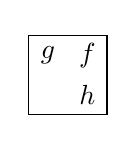
\begin{tikzpicture}[baseline=4mm]
\path (0,11mm) -- (1,1mm);
\draw (0,0) rectangle +(1,1);
\node at (.75,.25) {$h$};
\node at (.25,.75) {$g$};
\node at (.75,.75) {$f$};
\path (0,-1mm) -- (1,-1mm);
\end{tikzpicture}\,.
A figura~\ref{fig.astar2} mostra o mapa da grade após dois passos do algoritmo \astar{}. As células $(3,1)$ e $(3,0)$ recebem o mesmo custo $f$: uma está mais próxima de \p{S} (pelo número de passos contados) e a outra está mais próxima de \p{G} (pela heurística), mas ambas têm o mesmo custo de $7$.

O algoritmo precisa manter uma estrutura de dados das células abertas, as células que ainda não foram expandidas. Usamos a notação $(r,c,v)$, onde $r$ e $c$ são a linha e a coluna da célula e $v$ é o valor $f$ da célula. Cada vez que uma célula aberta é expandida, ela é removida da lista e as novas células são adicionadas. A lista é \emph{ordenada} para que as células com os valores mais baixos apareçam primeiro; isto facilita a decisão de qual célula expandir em seguida. As três primeiras listas correspondentes à Fig.~\ref{fig.astar2} são:
\begin{displaymath}
\begin{array}{l}
(4,0,5)\\
(4,1,5),\,(3,0,7)\\
(3,0,7),\,(3,1,7)\,.
\end{array}
\end{displaymath}

\begin{figure}
\begin{minipage}{.48\textwidth}
\begin{tikzpicture}[scale=.8]
\pic[scale=.8,draw] at (0,0) {astar};
\foreach \x/\y/\n in {0/0/5, 1/0/4, 0/1/6, 1/1/5, 0/2/7, 0/3/8, 1/2/6, 0/4/9, 1/3/7, 2/2/5, 3/2/4, 1/4/8, 3/3/5, 3/1/3, 3/4/6, 3/0/2, 4/1/2, 4/3/4, 4/0/1, 5/3/3, 4/4/5, 5/1/1, 5/4/4, 5/0/0}
  \node at (\x+.8,\y+.2) {\p{\n}};
\foreach \x/\y/\n in {0/0/0, 1/0/1, 0/1/1, 1/1/2, 0/2/2, 1/2/3, 2/2/4, 0/3/3, 1/3/4, 3/2/5, 3/3/6, 3/1/6}
  \node at (\x+.2,\y+.8) {\p{\n}};
\foreach \x/\y/\n in {0/0/5, 1/0/5, 0/1/7, 1/1/7, 0/2/9, 1/2/9, 2/2/9, 0/3/11, 1/3/11, 3/2/9, 3/3/11, 3/1/9}
  \node at (\x+.8,\y+.8) {\p{\n}};
\end{tikzpicture}
\caption{O algoritmo \astar{} após passos de $6$}
\label{fig.astar6}
\end{minipage}
\hspace{\fill}
\begin{minipage}{.48\textwidth}
\begin{tikzpicture}[scale=.8]
\foreach \x/\y in {0/0, 1/0, 1/1, 1/2, 2/2, 3/2, 3/1, 4/1, 5/1, 5/0}
  \draw[fill,lightgray] (\x,\y) rectangle +(1,1);
\pic[scale=.8,draw] at (0,0) {astar};
\foreach \x/\y/\n in {0/0/5, 1/0/4, 0/1/6, 1/1/5, 0/2/7, 0/3/8, 1/2/6, 0/4/9, 1/3/7, 2/2/5, 3/2/4, 1/4/8, 3/3/5, 3/1/3, 3/4/6, 3/0/2, 4/1/2, 4/3/4, 4/0/1, 5/3/3, 4/4/5, 5/1/1, 5/4/4, 5/0/0}
  \node at (\x+.8,\y+.2) {\p{\n}};
\foreach \x/\y/\n in {0/0/0, 1/0/1, 0/1/1, 1/1/2, 0/2/2, 1/2/3, 2/2/4, 0/3/3, 1/3/4, 3/2/5, 3/3/6, 3/1/6, 3/0/7, 4/1/7, 4/0/8, 5/1/8, 5/0/9}
  \node at (\x+.2,\y+.8) {\p{\n}};
\foreach \x/\y/\n in {0/0/5, 1/0/5, 0/1/7, 1/1/7, 0/2/9, 1/2/9, 2/2/9, 0/3/11, 1/3/11, 3/2/9, 3/3/11, 3/1/9, 3/0/9, 4/1/9, 4/0/9, 5/1/9, 5/0/9}
  \node at (\x+.8,\y+.8) {\p{\n}};
\end{tikzpicture}
\caption{O algoritmo \astar{} alcança a célula de objetivo e encontra um caminho mais curto}
\label{fig.astar9}
\end{minipage}
\end{figure}


%\begin{figure}
%\subfigures
%\begin{minipage}{\textwidth}
%\leftfigure[c]{
%\begin{tikzpicture}[scale=.8]
%\pic[scale=.8] at (0,0) {astar};
%\foreach \x/\y/\n in {0/0/5, 1/0/4, 0/1/6, 1/1/5, 0/2/7, 0/3/8, 1/2/6, 0/4/9, 1/3/7, 2/2/5, 3/2/4, 1/4/8, 3/3/5, 3/1/3, 3/4/6, 3/0/2, 4/1/2, 4/3/4, 4/0/1, 5/3/3, 4/4/5, 5/1/1, 5/4/4, 5/0/0}
%  \node at (\x+.8,\y+.2) {\p{\n}};
%\foreach \x/\y/\n in {0/0/0, 1/0/1, 0/1/1, 1/1/2, 0/2/2, 1/2/3, 2/2/4, 0/3/3, 1/3/4, 3/2/5, 3/3/6, 3/1/6}
%  \node at (\x+.2,\y+.8) {\p{\n}};
%\foreach \x/\y/\n in {0/0/5, 1/0/5, 0/1/7, 1/1/7, 0/2/9, 1/2/9, 2/2/9, 0/3/11, 1/3/11, 3/2/9, 3/3/11, 3/1/9}
%  \node at (\x+.8,\y+.8) {\p{\n}};
%\end{tikzpicture}
%}
%\hspace{\fill}
%\rightfigure[c]{
%\begin{tikzpicture}[scale=.8]
%\foreach \x/\y in {0/0, 1/0, 1/1, 1/2, 2/2, 3/2, 3/1, 4/1, 5/1, 5/0}
%  \draw[fill,lightgray] (\x,\y) rectangle +(1,1);
%\pic[scale=.8] at (0,0) {astar};
%\foreach \x/\y/\n in {0/0/5, 1/0/4, 0/1/6, 1/1/5, 0/2/7, 0/3/8, 1/2/6, 0/4/9, 1/3/7, 2/2/5, 3/2/4, 1/4/8, 3/3/5, 3/1/3, 3/4/6, 3/0/2, 4/1/2, 4/3/4, 4/0/1, 5/3/3, 4/4/5, 5/1/1, 5/4/4, 5/0/0}
%  \node at (\x+.8,\y+.2) {\p{\n}};
%\foreach \x/\y/\n in {0/0/0, 1/0/1, 0/1/1, 1/1/2, 0/2/2, 1/2/3, 2/2/4, 0/3/3, 1/3/4, 3/2/5, 3/3/6, 3/1/6, 3/0/7, 4/1/7, 4/0/8, 5/1/8, 5/0/9}
%  \node at (\x+.2,\y+.8) {\p{\n}};
%\foreach \x/\y/\n in {0/0/5, 1/0/5, 0/1/7, 1/1/7, 0/2/9, 1/2/9, 2/2/9, 0/3/11, 1/3/11, 3/2/9, 3/3/11, 3/1/9, 3/0/9, 4/1/9, 4/0/9, 5/1/9, 5/0/9}
%  \node at (\x+.8,\y+.8) {\p{\n}};
%\end{tikzpicture}
%}
%\leftcaption{The \astar{} algorithm after $6$ steps\label{fig.astar6}}
%\rightcaption{The \astar{} algorithm reaches the goal cell and finds a shortest path\label{fig.astar9}}
%\end{minipage}
%\end{figure}

A figura~\ref{fig.astar6} mostra o mapa da grade após seis etapas. Isto pode ser visto observando os valores de $g$ no canto superior esquerdo de cada célula. A lista atual de células abertas é:
\[
(3,3,9),\, (1,0,11),\, (1,1,11),\, (1,3,11)\,.
\]
O algoritmo \astar{} escolhe expandir a célula $(3,3,9)$ com os menores $f$. As outras células da lista têm um valor de $f$ de $11$ e são ignoradas pelo menos por enquanto. Continuando (Fig.~\ref{fig.astar9}), a célula de objetivo é atingida com o valor $f$ $9$ e um caminho mais curto em cinza é exibido. A última lista antes de atingir a meta é:
\[
(3,5,9),\, (4,4,9),\, (1,0,11),\, (1,1,11),\, (1,3,11)\,.
\]
Não importa qual dos nós com valor $9$ é escolhido: em ambos os casos, o algoritmo atinge a célula de objetivo $(4,5,9)$.

Todas as células da parte superior direita da grade não são exploradas porque a célula $(1,3)$ tem valor $f$ $11$ e este nunca será o menor valor. Enquanto o algoritmo de Dijkstra explorou todas as células não-obstáculos de $24$, o algoritmo \astar{} explorou apenas células de $17$.

\subsubsection*{Um exemplo mais complexo do algoritmo \astar}

Vamos aplicar o algoritmo \astar{} ao mapa da grade na Fig.~\ref{fig.path-sand}. Lembre-se que este mapa tem areia em algumas de suas células, portanto a função $g$ dará valores mais altos para o custo da mudança para estas células. O diagrama superior esquerdo da Fig.~\ref{fig.a-star} mostra a função $g$ como computada pelo algoritmo de Dijkstra, enquanto o diagrama superior direito mostra a função heurística $h$, o número de passos da meta na ausência de obstáculos e a areia. O restante da figura mostra quatro estágios do algoritmo que conduzem ao caminho mais curto para o objetivo.

\begin{figure}
\begin{center}
\includegraphics[width=0.8\textwidth]{a-star-sand.pdf}
\end{center}
\caption{O algoritmo \astar{}. Na parte superior esquerda: o número de passos para o objetivo. Em cima à direita: a função heurística. Os diagramas do meio e inferior mostram quatro passos do algoritmo.}\label{fig.a-star}
\end{figure}

Já a partir do diagrama do meio esquerdo, vemos que não é necessário procurar em direção ao topo esquerdo, pois os valores de $f$ das células acima e à esquerda de \p{S} são maiores que os valores à direita e abaixo de \p{S}. No diagrama do meio direito, a primeira célula de areia tem um valor de $13$, então o algoritmo continua a expandir as células com o menor custo de $12$ para a esquerda. No diagrama inferior esquerdo, vemos que a busca não continua para a esquerda inferior do mapa porque o custo de $16$ é maior do que o custo de $14$ uma vez que a busca deixa a areia. A partir desse ponto, a célula de objetivo \p{G} é encontrada muito rapidamente. Como no algoritmo de Dijkstra, o caminho mais curto é encontrado traçando de volta através de células com valores mais baixos de $g$ até que a célula inicial seja alcançada.

Comparando Figs.~\ref{fig.dijkstra} e \ref{fig.a-star} vemos que o algoritmo \astar{} precisava visitar apenas 71\% das células visitadas pelo algoritmo de Dijkstra. Embora o algoritmo \astar{} do Dijkstra deva realizar um trabalho adicional para calcular a função heurística, o número reduzido de células visitadas torna o algoritmo mais eficiente. Além disso, esta função heurística depende apenas da área pesquisada e não dos obstáculos; mesmo que o conjunto de obstáculos seja alterado, a função heurística não precisa ser recalculada.

\begin{framed}
\act{Algoritmo A*}{astar}
\begin{itemize}
\item Aplique o algoritmo \astar{} e o algoritmo de Dijkstra em um pequeno mapa sem obstáculos: coloque a célula inicial no centro do mapa e o objetivo em uma célula arbitrária. Compare os resultados dos dois algoritmos. Explique seus resultados. O resultado depende da posição da célula de objetivo?
\item Definir outras funções heurísticas e comparar os resultados dos algoritmos de \astar{} sobre os exemplos deste capítulo.
\end{itemize}
\end{framed}

\section{Seguir o caminho e evitar obstáculos}\label{s.path-and-obstacle}

Este capítulo e os anteriores discutiram duas tarefas diferentes, mas relacionadas: planejamento de caminhos de alto nível e evitar obstáculos de baixo nível. Como integrar os dois? A abordagem mais simples é priorizar o algoritmo de baixo nível (Fig.~\ref{fig.integrate-pp}). Obviamente, é mais importante evitar bater em um pedestre ou dirigir ao redor de um buraco do que tomar o caminho mais curto até o aeroporto. O robô normalmente está em seu estado \p{drive}, mas se for detectado um obstáculo, ele faz uma transição para o estado de \p{evitar obstáculo}. Somente quando o obstáculo tiver sido passado, ele retorna para o estado de "caminho do plano", para que o caminho possa ser recalculado.

\begin{figure}
\begin{center}
\begin{tikzpicture}[scale=.8,node distance = 2cm and 4cm,align=left,minimum size=16mm]
\node[draw,circle] (plan)  {\p{plan}\\\p{path}};
\node[draw,circle] (drive) [right=of plan] {\p{drive}};
\draw[->] (plan) to node[above,yshift=-4mm] {\p{true }$\leadsto$ \\ \p{move to goal}} (drive);
\draw[<-] (plan) to (180:15mm);
\node[draw,circle] (avoid) [below=of drive] {\p{avoid}\\\p{obstacle}};
\draw[->] (drive) to node[left,yshift=2mm] {\p{obstacle detected} $\leadsto$ \\ \p{move around obstacle}} (avoid);
\draw[->,bend left=20] (avoid) to node[left,xshift=-6mm] {\p{obstacle passed} $\leadsto$\\\p{[no action]}} (plan);
\end{tikzpicture}
\caption{Integrando o planejamento de caminhos e evitando obstáculos}\label{fig.integrate-pp}
\end{center}
\end{figure}

A estratégia para integrar os dois algoritmos depende do ambiente. O conserto de uma estrada pode levar várias semanas, portanto, faz sentido acrescentar o obstáculo ao mapa. O algoritmo de planejamento do trajeto levará em conta o obstáculo e o trajeto resultante provavelmente será melhor do que aquele que é alterado no último minuto por um algoritmo para evitar obstáculos. No outro extremo, se houver muitos obstáculos em movimento, como pedestres atravessando uma rua, o comportamento de evitar obstáculos pode ser simplesmente parar de se mover e esperar até que os obstáculos se afastem. Então, o plano original pode ser simplesmente retomado sem desvios.

\begin{framed}
\act{Combinando o planejamento de caminhos e a prevenção de obstáculos}{combi}
\begin{itemize}
\item Modifique sua implementação do algoritmo de acompanhamento de linha para que o robô se comporte corretamente mesmo que um obstáculo seja colocado na linha. Tente várias das abordagens listadas nesta seção.
\item Modifique sua implementação do algoritmo de seguimento de linha para que o robô se comporte corretamente mesmo que robôs adicionais estejam se movendo aleatoriamente na área da linha. Certifique-se de que os robôs não esbarrem uns nos outros.
\end{itemize}
\end{framed}

\section{Sumário}

O planejamento do caminho é um comportamento de alto nível de um robô móvel: encontrar o caminho mais curto desde um local inicial até um local de objetivo no ambiente. O planejamento do trajeto é baseado em um mapa que mostra os obstáculos. O algoritmo de Dijkstra expande o caminho mais curto para qualquer célula encontrada até agora. O algoritmo \astar{} reduz o número de células visitadas usando uma função heurística que indica a direção para a célula de objetivo.

O planejamento do caminho é baseado em um gráfico como um mapa de grade, mas também pode ser feito em um mapa contínuo, criando um gráfico de obstáculos a partir do mapa. Os algoritmos podem levar em conta os custos das variáveis para visitar cada célula.

A prevenção de obstáculos de baixo nível deve ser integrada no planejamento de caminhos de alto nível.

\section{Leitura adicional}

O algoritmo de Dijkstra é apresentado em todos os livros de texto sobre estruturas de dados e algoritmos, por exemplo, \cite[Sect.~24.3]{crls3}. Algoritmos de busca como o algoritmo \astar{} são um tópico central da inteligência artificial \cite[Sect.~3.5]{ai}.
